\section{Methods and materials}
\begin{itemize}
\item 1 six-year old grapefruit plant
\item 1 cord of known spring constant
\item 1 measuring tape
\item 1 Kaz Inc. Ht-908 15 inch Honeywell Turbo Force Room Air Circulator Fan
\item colored construction paper
\item 1 pair of scissors
\item clear tape
\item 1 Samsung Galaxy S-8 smartphone camera
\item 1 wooden chair
\item flat, rectangular surfaces
\item MATLAB software
\item pipe cleaners
\item nylon rope
\end{itemize}

	The first step in the process was to find a cord of known spring constant. In this experiment, a cord from a party mask was found to have a spring coefficient of \SI{1.03}{\newton\per\centi\meter}. The cord was attached to a nylon rope and tied to pipe cleaners at both ends so that it could be connected to plant stems. The pipe cleaners were included in the spring constant calculation.

	The experimental setup for measuring the spring's deflection due to drag is shown in \fref{fig:methods1}. The cord was strung between a heavy chair and the trunk of a grapefruit plant so that it was not slack, and its length was measured using a tape measure. Then, a box fan was placed one foot away from the trunk of the plant. The plant and fan were raised using flat, rectangular objects, such as textbooks, in order to position the plant's canopy in front of the fan. The cord's deflection was measured five times at each of the fan's three speed settings and a slow motion video of the plant's leaves was taken at the highest fan setting.

Next, the cross sectional area of the plant was calculated using color blob detection in Matlab. To do this, black construction paper was cut to the size and shape of the fan's opening and affixed to it. Because air was blowing from relatively close to the plant, only the area which was directly in front of the fan opening would be exposed to wind. The plant was of a complex shape, so it was more efficient to calculate the area of the fan which was not covered by the plant. The setup was photographed from afar and scaled to eliminate the colorful surroundings, as shown in appendix~\ref{app:A}. A picture of the fan-shaped paper was also taken against a blue background from the same distance with no citrus obscuring it and scaled by the same amount, which can also be seen in appendix~\ref{app:A}. Using Matlab's \lstinline{colorThresholder} system, the ratio of covered to uncovered area was found and multiplied by the known paper area to find the area of the grapefruit leaves.

After analyzing the results of the grapefruit plant, a rigid model of a single leaf was created to test the same conditions without the presence of bending. A small leaf was placed against an aluminum Chipotle bowl lid to serve as a stencil, which was cut out using scissors. Then, this model leaf was taped to a wooden pencil so that the pencil would prevent it from flexing, while any tape edges were cut off. The finished leaf model can be seen in \fref{fig:methods2}. 

The leaf model was tested in the same manner as the grapefruit plant at the highest fan setting. Because the deflection in the cord was quite small, the displacement was measured using slow motion video. To do this, a tape measure with millimeters marked was taped below the cord and the video was taken from directly above. The video device was planted on a solid surface to minimize movement, and the displacement was found by zooming in on the video and pausing when the cord was fully extended and relaxed. The experimental setup for the model can be seen in \fref{fig:methods3}.

In order to compare the model area to the area of the grapefruit, a sheet of orange construction paper was photographed with and without the model leaf against it. Then, using the color blob detection technique in Matlab, the ratio of the model area to the paper area was calculated and multiplied by the actual paper area, in square feet. The images for this analysis can be seen in appendix~\ref{app:A}.

With the approximate cross sectional areas of the actual grapefruit leaves and the model found, the discussion over how these areas and their corresponding drags differed could begin.


% Fig 1 is good but cluttered, can we zoom in on only the business part; or turn it into a drawing. Altnatively, add callouts and scale bar? Is there a shot more from the side, that shows the experimental rig without foreshortening? 
% Agreed, I'll put in a drawing instead to make it neater
\begin{figure}
\begin{center}
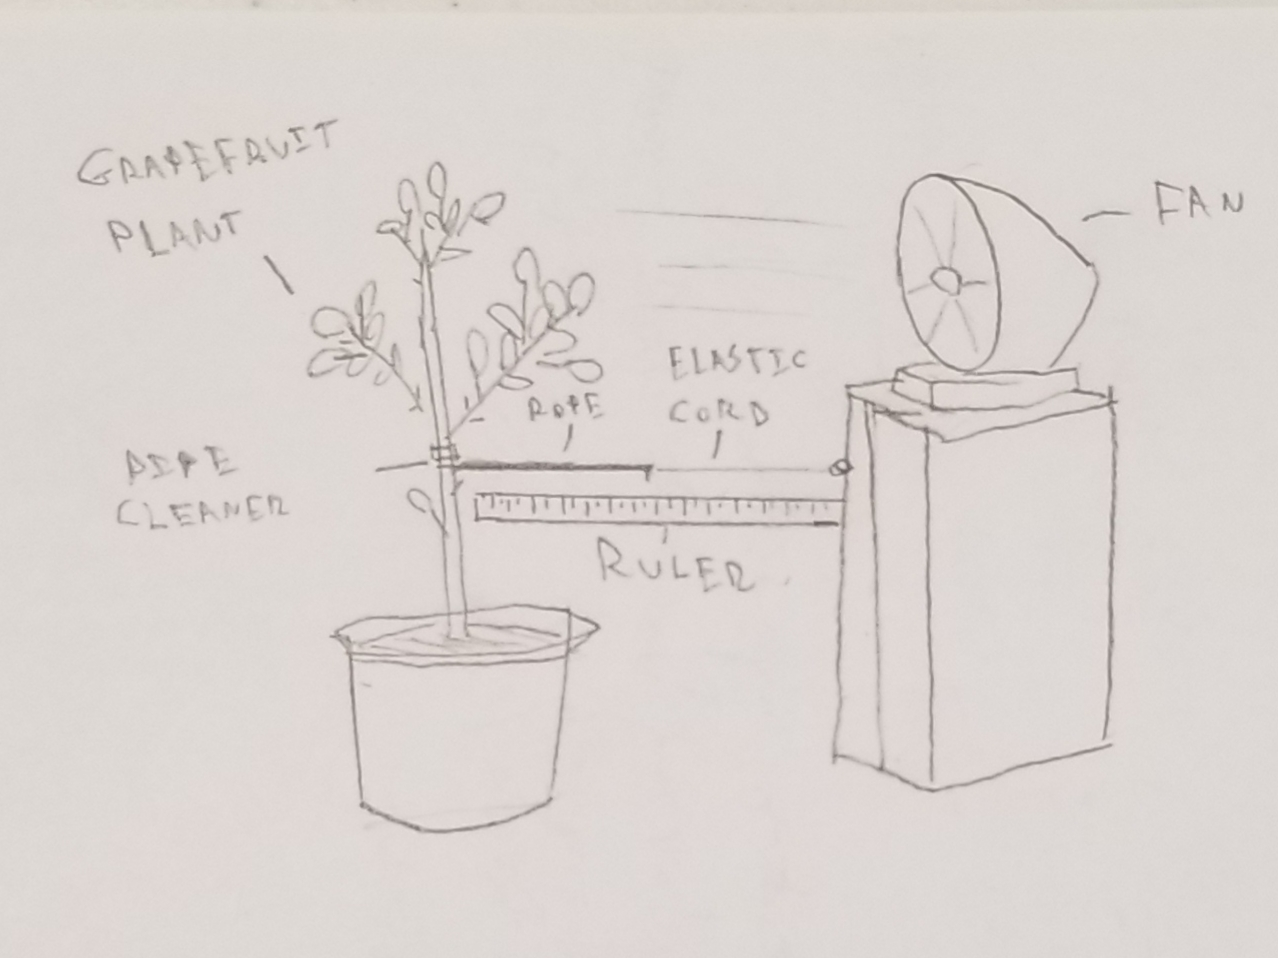
\includegraphics[width=0.5\columnwidth]{figures/Setup1.jpg} 
\end{center}
\caption{Experimental setup to measure the deflection of a grapefruit plant when exposed to wind.}
\label{fig:methods1}
\end{figure}

% Fig 2 is good but zoom in on the two, add callouts and a scalebar, maybe rotate leaves into their normal positions. 
\begin{figure}
\begin{center}
\includegraphics[width=0.33\columnwidth]{figures/Metal_Leaf_Compared.jpg}
\includegraphics[width=0.33\columnwidth]{figures/Measured Model.jpg}
\end{center}
\caption{The aluminum grapefruit leaf model (left) with a small jackfruit leaf. Measuring tape (cm) along the model, for scale (right).}
\label{fig:methods2}
\end{figure}

\begin{figure}
\begin{center}
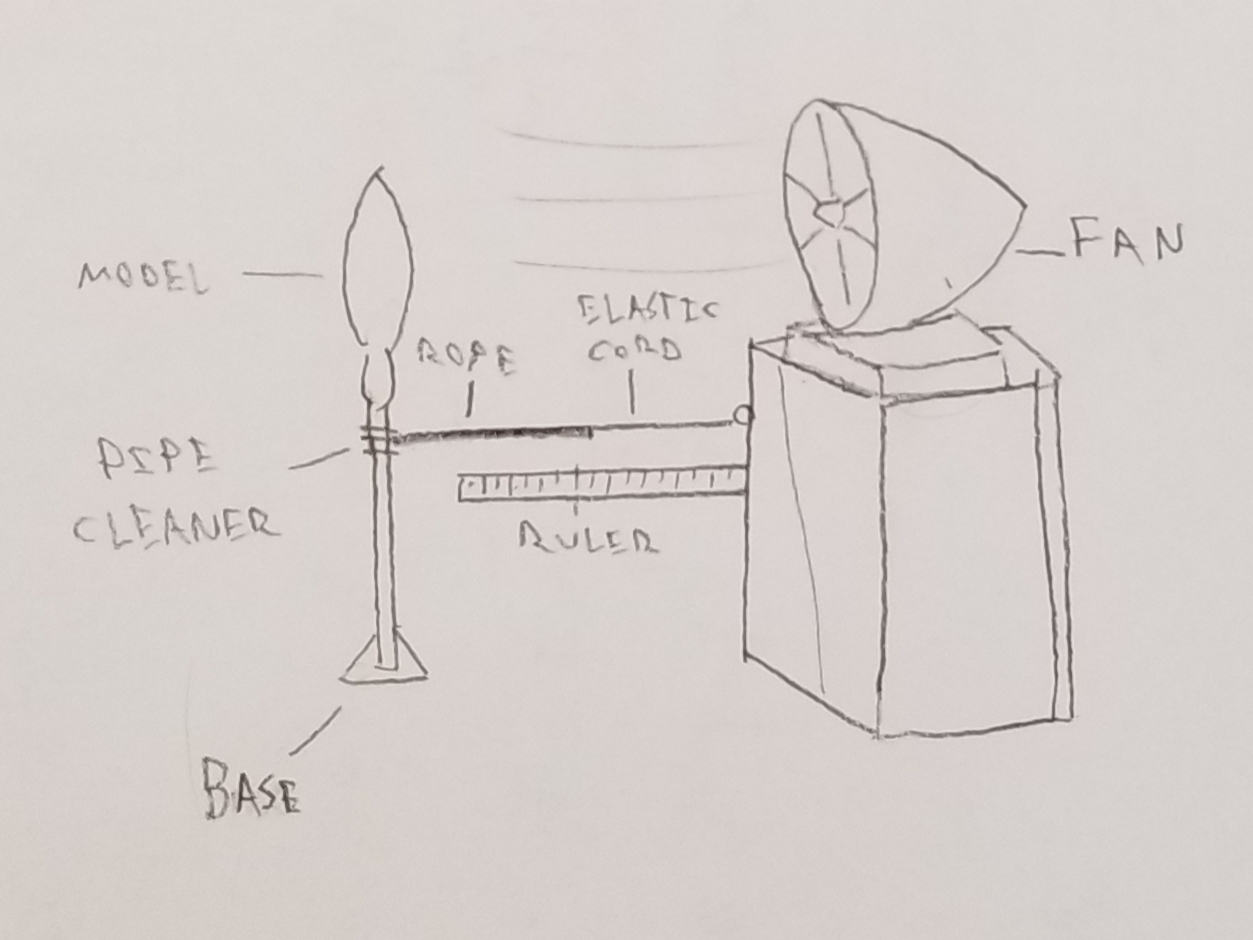
\includegraphics[width=0.5\columnwidth]{figures/Setup2.jpg}
\end{center}
\caption{The setup for testing the rigid model drag when exposed to wind.}
\label{fig:methods3}
\end{figure}




\subsection{Specimens and physical models}
I used a single \SI{6}{y} old specimen of \Citrusxparadisi\ (grapefruit) for all measurements. This specimen was germinated in Toledo, Ohio in January of 2014. As it grew, it spent its summers in the bright outdoors and winters in the relatively dark indoors, staying in a plastic pot throughout its life. This caused it to grow top heavy, with larger leaves in the canopy and smaller leaves in its understory. Additionally, it was subject to attacks from Tetranychid mites each winter, leaving many leaves scarred. At the time of these trials, the specimen had just ended its winter indoor period, causing it to experience rapid growth. It stood at \SI{41}{in} tall and measured \SI{25}{in} across at its widest point. The wind tunnel analysis was focused on the plant's disproportionately large top.

To remove the effects of flexibility, I also created a physical model of a single \Cxparadisi\ leaf using \SI{0.1}{\milli\meter} thick aluminum sheeting from a food container (Chipotle; 6658 Airport Hwy ste c, Holland, OH 43528). To prepare the physical model, I traced an actual leaf and cut the profile of the model to match. The physical model was mounted on a wooden pencil to provide a rigid attachment point compared to the typical flexible leaf petioles on \Cxparadisi. The finished product can be seen in \fref{fig:methods2}.

\subsection{Statistical analyses}
Statistical analyses of the effects of both leaf and fan speed on drag and drag/area were performed using R \citep{r2020} using two-way analysis of variance (ANOVA); plots were prepared using the \lstinline{tidyverse} and \lstinline{ggplot2} libraries \citep{wickham2019tidyverse}.

Applying the percent difference formula

\[D=100*\frac{2*|V1-V2|}{|V1-V2|}\]
yields a difference of 17 percent between the drag to area ratios of the model and the actual plant at fan setting 3. 








